\documentclass{article}

% variables
\newcommand{\doctitle}{Creación y manejo de procesos}
\newcommand{\docauthor}{Milton Hernández M.}
\newcommand{\docnumber}{001}
\newcommand{\refnumber}{001}
\newcommand{\versionnumber}{1.0}
\newcommand{\revisionnumber}{1}
\newcommand{\changeregister}{001}
\newcommand{\doctype}{Práctica }
\newcommand{\docdate}{30 de Septiembre del 2024}
\newcommand{\docyear}{2024}
\newcommand{\doctime}{10:00 Pm}
\newcommand{\docsubject}{Introducción a Sistemas Operativos}
\newcommand{\docprofessor}{Eduardo Peña J.}

% Paquetes para codificación y lenguaje
\usepackage[utf8]{inputenc}                            % Codificación
\usepackage[english, spanish]{babel}                   % Lenguaje
\usepackage{csquotes}                                  % COmpatibilidad con BibLatex
\spanishdecimal{.}                                     % Punto decimal

% Paquetes para matemáticas
\usepackage{amsmath, amsthm, amssymb}                  % Matemáticas
\usepackage{mathptmx}

% Paquetes para geometría y diseño de página
\usepackage[margin=2.5cm, headheight=2cm]{geometry}    % Márgenes

% Paquetes para gráficos y figuras
\usepackage{graphicx}                                  % Imágenes
\usepackage{wrapfig}                                   % Figuras a la derecha

% Paquetes para hipervínculos
\usepackage{hyperref}                                  % Hipervínculos
\hypersetup{
    colorlinks=true,
    linkcolor=black,
    urlcolor=blue,
    citecolor=blue,
}

% Paquetes para encabezados y pies de página
\usepackage{fancyhdr}
\pagestyle{fancy}

% Encabezado y pie de página
\rhead{\doctitle}
\lhead{}
\cfoot{}
\rfoot{\thepage}

% Paquetes adicionales
\usepackage{mhchem}                                    % Química
\usepackage{siunitx}                                   % Notación científica
\sisetup{%
	detect-family,
	per-mode = fraction,
	%per-mode = symbol,
	separate-uncertainty = true,
	%output-decimal-marker = {,}
	%exponent-product = \cdot,
	inter-unit-product =\cdot
}
\DeclareSIUnit\atm{Atm}
\DeclareSIUnit\molar{M}
\usepackage{caption}
\usepackage{xcolor}                                    % Colores personalizados
	\definecolor{codegreen}{rgb}{0,0.5,0}
	\definecolor{codegray}{rgb}{0.5,0.5,0.5}
	\definecolor{codepurple}{rgb}{0.5,0,0.5}
	\definecolor{backcolour}{rgb}{0.95,0.95,0.95}
\usepackage{booktabs}                                  % Tablas mejoradas
\usepackage{multirow}
\usepackage{listings}                                  % Para código
\usepackage[backend=biber,style=apa]{biblatex}         % Bibliografía
\addbibresource{referencias.bib}


% Otras configuraciones
\setlength{\parindent}{0pt}                               % Indentación
\setlength{\parskip}{7pt}                                  % Espaciado entre párrafos
\renewcommand{\baselinestretch}{1.5}                       % Interlineado
\addto\captionsspanish{\renewcommand{\tablename}{Tabla}}   % Redefinir el nombre de la tabla
\addto\captionsspanish{\renewcommand{\figurename}{Figura}} % Redefinir el nombre de la tabla

% Definir el estilo para el código
\lstdefinestyle{CodeStyle}{
    backgroundcolor=\color{backcolour},
    commentstyle=\color{codegreen},
    keywordstyle=\color{codepurple},
    numberstyle=\tiny\color{codegray},
    stringstyle=\color{codepurple},
    basicstyle=\ttfamily\footnotesize,
    breakatwhitespace=false,
    breaklines=true,
    captionpos=t,
    keepspaces=true,
    numbers=left,
    numbersep=5pt,
    showspaces=false,
    showstringspaces=false,
    showtabs=false,
    tabsize=2
}

\begin{document}

\begin{titlepage}
    \centering
    \begin{center}
        
\includegraphics[width=0.8\textwidth]{src/images/Depto_compu.png}
    \end{center}
    \vspace{0.01cm}
    {\LARGE\bfseries \doctitle \par}
    {\large\doctype No° \docnumber\par}
    \vspace{1.5cm}
    {\large \textbf{Estudiante:} Milton Hernández - \href{mailto:milherna@umag.cl}{milherna@umag.cl}}\\
    \vspace{0.3cm}
    \textbf{Fecha y hora:} {\docdate - \doctime} \\
    \vspace{0.3cm}
    {\large \textbf{Profesor:} \docprofessor \par}
    \vspace{0.3cm}
    {\large \textbf{Asignatura:} \docsubject \par}
    \vspace{1.5cm}
    {\LARGE\bfseries Status del documento \par}
    \begin{table}[!ht]
    \centering
    \begin{tabular}{|cccc|}
    \hline
    \multicolumn{4}{|c|}{\textbf{\begin{tabular}[c]{@{}c@{}}\doctype N°\docnumber\\ \doctitle\end{tabular}}}                                               \\ \hline
    \multicolumn{3}{|c|}{\textbf{\begin{tabular}[c]{@{}c@{}}Número de referencia\\ del documento\end{tabular}}} & \docnumber                            \\ \hline
    \multicolumn{1}{|c|}{\textbf{Versión}} & \multicolumn{1}{c|}{\textbf{Revisión}} & \multicolumn{1}{c|}{\textbf{Fecha}} & \textbf{Razones del cambio} \\ \hline
    \multicolumn{1}{|c|}{\versionnumber}          & \multicolumn{1}{c|}{\revisionnumber}         & \multicolumn{1}{c|}{\docdate}         & Primera revisión del documento \\ \hline
    \end{tabular}
\end{table}
    \vfill
\end{titlepage}
\newpage

% Please add the following required packages to your document preamble:
% \usepackage{multirow}
\begin{table}[!ht]
  \centering
  \begin{tabular}{|cccc|}
  \hline
  \multicolumn{2}{|c|}{\multirow{4}{*}{\textbf{\begin{tabular}[c]{@{}c@{}}Registro de\\ cambios del\\ documento\end{tabular}}}} &
  \multicolumn{1}{c|}{\textbf{RCD N°:}}        &  \changeregister                                                   \\ \cline{3-4}
  \multicolumn{2}{|c|}{}                         & \multicolumn{1}{c|}{\textbf{Fecha:}}         & \docdate          \\ \cline{3-4}
  \multicolumn{2}{|c|}{}                         & \multicolumn{1}{c|}{\textbf{Otiginado por:}} & \docauthor \\ \cline{3-4}
  \multicolumn{2}{|c|}{}                         & \multicolumn{1}{c|}{\textbf{Aprobado por:}}  & \docauthor \\ \hline
  \multicolumn{2}{|c|}{\textbf{Titulo del documento:}} &
    \multicolumn{2}{c|}{\begin{tabular}[c]{@{}c@{}}\doctype N°\docnumber\\ \doctitle \end{tabular}} \\ \hline
  \multicolumn{3}{|c|}{\textbf{Número de referencia del documento:}}                            & \refnumber                 \\ \hline
  \multicolumn{1}{|c|}{\textbf{Versión del documento}} &     \multicolumn{1}{c|}{\versionnumber} &
  \multicolumn{1}{c|}{\textbf{Número de revisión:}}    &     \revisionnumber \\ \hline
  \multicolumn{1}{|c|}{\textbf{Página}} &
    \multicolumn{1}{c|}{\textbf{Párrafo}} &
    \multicolumn{2}{c|}{\textbf{Razones del cambio}} \\ \hline
  \multicolumn{1}{|c|}{} & \multicolumn{1}{c|}{} & \multicolumn{2}{c|}{}                                              \\ \hline
  \multicolumn{1}{|c|}{} & \multicolumn{1}{c|}{} & \multicolumn{2}{c|}{}                                              \\ \hline
  \multicolumn{1}{|c|}{} & \multicolumn{1}{c|}{} & \multicolumn{2}{c|}{}                                              \\ \hline
  \multicolumn{1}{|c|}{} & \multicolumn{1}{c|}{} & \multicolumn{2}{c|}{}                                              \\ \hline
  \end{tabular}
\end{table}
\newpage

\tableofcontents
\newpage

\begin{abstract}
    La comunicación y sincronización entre procesos es una de las tareas más delicadas a la hora de trabajar con Sistemas Operativos, esto debido a que una mala gestión de este ámbito podría ocasionar pérdidas de información, procesos bloqueados permanentemente e incluso la proliferación de malware en el equipo. Por esta razón, desde los inicios de la computación, se han desarrollado diversas técnicas para dar un correcto manejo a la comunicación y sincronización de procesos y la comunicación de los mismos algunas de las cuales serán puestas a prueba en la realización del presente informe.
\end{abstract}
\input{src/sections/introducción.tex}
\section{Objetivo Principal}
Comprender el funcionamiento de la \textbf{Transferencia de mensajes} como método de comunicación entre procesos y su implementación en \texttt{C}.

\section{Objetivos secundarios}
\begin{enumerate}
    \item Investigar la manera correcta de crear un enlace de comunicación entre dos procesos mediante el uso de colas de mensajes en \texttt{C}.
    \item Analizar el funcionamiento de la Transferencia de mensajes entre más de dos procesos, generando grupos de productores de mensajes y consumidores de mensajes.
\end{enumerate}
\newpage

\section{Marco teórico}
El marco teórico se divide en tres secciones: la primera describe el funcionamiento de los procesos dentro de un sistema operativo, y la segunda aborda la creación de procesos concurrentes y la tercera ahondará un poco en la creación de objetos aleatorios dentro de un sistema computarizado.

\subsection{Funcionamiento de los procesos dentro de un sistema operativo}
Como hemos mencionado anteriormente los procesos se pueden definir como programas que se ejecutan dentro de un sistema operativo.

Cabe mencionar que un proceso puede pasar por distintos estados durante su ejecución, algunos de estos estados son:
\begin{itemize}
    \item \textbf{Proceso nuevo:} Cuando un proceso es creado por algún medio este se encuentra en estado nuevo.
    \item \textbf{En ejecución:} Un proceso está en ejecución cuando la CPU se encuentra procesando información a su respecto en un instante determinado de tiempo.
    \item \textbf{En pausa:} cuando el proceso es suspendido temporalmente por el sistema operativo este se pone en pausa, a la espera de poder continuar su ejecución. (Estas pausas pueden llegar a durar muy pocos milisegundos).
    \item \textbf{Bloqueado:} se refiere a cuando un proceso está esperando que ocurra un evento externo, como la disponibilidad de un recurso. En este estado el proceso puede durar más tiempo que en una pausa e incluso puede no volver a ejecutarse.
    \item \textbf{Terminado:} Cuando todas las tareas relacionadas con un proceso se han completado este proceso se encuentra en estado terminado.
\end{itemize}

Podemos ver un gráfico del comportamiento de estos estados en la figura~\ref{fig:estadosDeProcesos}.

\begin{figure}[!ht]
    \centering
    \caption{Estados de los procesos}
    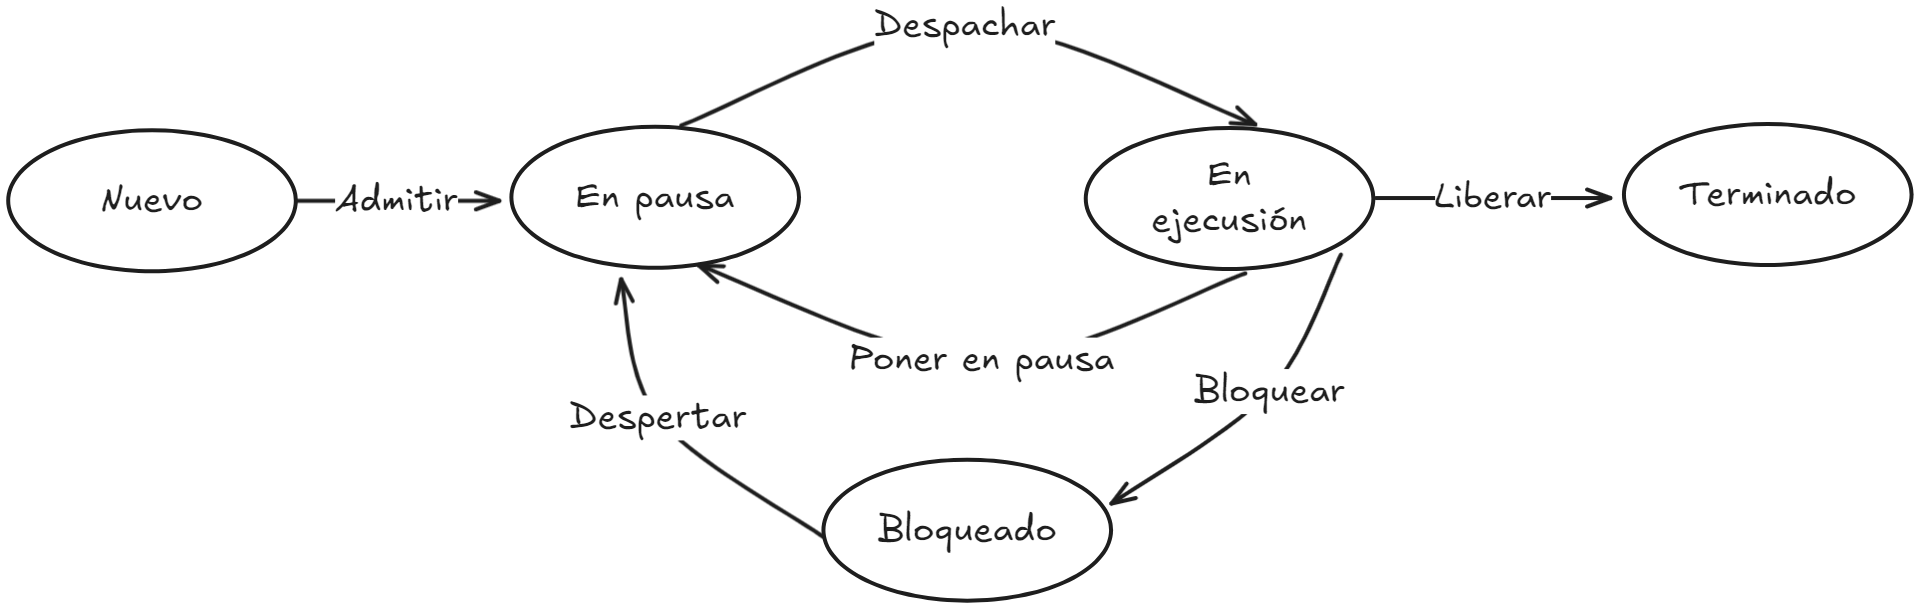
\includegraphics[width=0.9\textwidth]{src/images/Estados de procesos.png}\label{fig:estadosDeProcesos}
\end{figure}

Comprender los diferentes estados de un proceso así como el hecho de que al ejecutar en un mismo periodo varios procesos lo que ocurre realmente es que la CPU se encarga de ejecutar cada uno de ellos en un corto periodo en un orden determinado. (Como explicado en la introducción) es el fundamento del presente laboratorio.

\subsection{Creación de procesos concurrentes dentro de un sistema operativo}
Trabajar con procesos concurrentes dentro de un sistema operativo puede ser complejo si no se cuenta con los conocimientos necesarios para su creación y manejo.

Supongamos que, como se realizará posteriormente, tenemos tres programas encargados de la generación de productos de manera continua (números, letras, etc) y que deseamos ejecutarlos de manera paralela o, como se mencionará en adelante \textbf{de manera distendida}.

En caso de trabajar en un sistema Linux (como es el caso del presente laboratorio) para ejecutar los procesos en segundo plano, se puede usar el comando $\&$, lo que permite que el proceso continúe su ejecución mientras la consola queda disponible para otras tareas.

\begin{lstlisting}[language=bash, style=CodeStyle]
$ ./Generador_uno &
$ ./Generador_dos &
$ ./Generador_tres &
\end{lstlisting}

Esto indica que el proceso generador\_uno se ejecutará en segundo plano, lo mismo para el generador\_2 y para el generador\_tres. Al final de esta ejecución la consola quedará libre para poder continuar con otras tareas.

Para poder ver los procesos en ejecución y eliminarlos es necesario utilizar el comando \textit{ps} que nos devuelve una lista de todos los procesos en ejecución del sistema operativo.

\begin{lstlisting}[language=bash, style=CodeStyle]
$ ps
  PID TTY          TIME CMD
  101 pts/0    00:00:00 bash
  102 pts/0    00:00:00 ps
\end{lstlisting}

<<\textit{Si introduces el comando ps sin opciones, únicamente te mostrará los procesos iniciados por el shell actual. Por lo tanto, otros procesos quedan excluidos inicialmente.}>> \parencite{PS}.

Durante el presente informe se realizarán varios programas para su posterior ejecución mediante el uso del lenguaje C como veremos en el Procedimiento Experimental.

\subsection{Creación de números aleatorios}
<<\textit{Por naturaleza, las computadoras no son muy buenas con el azar. Su fortaleza radica en generar salidas predecibles ejecutando secuencias de operaciones programadas. Eso es casi lo opuesto a la aleatoriedad.}>> \parencite{NumerosAleatorios}.

De acuerdo con \textcite{eduardo2022Azar} el mejor método de generación de números aleatorios se encuentra en los sistemas cuánticos como el usado por la web \href{https://www.random.org/}{random.org}. Sin embargo no es muy cómodo tener que recurrir a información externa a un equipo para generar números aleatorios, por lo cuál se crearon con el tiempo algoritmos que generan números llamados \textbf{Pseudo Aleatorios}, es decir números que detrás llevan un desarrollo no aleatorio pero que a los ojos de los comsumidores lo son.

Una de las maneras de generar números de este tipo es mediante la técnica \textbf{LFSR} que se traduce al español como: \textit{registro de desplazamiento con retroalimentación lineal} que utiliza funciones lógicas sencillas y por tanto es muy sencilla de programar y de implementar a nivel del Hardware. El proceso consiste en lo siguiente:
\begin{enumerate}
  \item Se inicia con una semilla en binario.
  \item En cada repetición del proceso de cálculo se saca el último bit del número semilla.
  \item Posteriormente el resto de bits se corren a la derecha.
  \item En el espacio sobrante se agrega un bit, resultado de una operación lógica realizada sobre los bits restantes.
  \item Este proceso se repite, generando con los bits que se van retirando un número binario que se puede entregar como \"aleatorio\".
\end{enumerate}

Como se ve el procedimiento depende de la semilla usada; en caso de usar la misma semilla los resultados serán iguales, por lo que se precisa de una manera certera de crear semillas con las que alimentar este generador de pseudo-aleatoriedad.

Los diferentes lenguajes de programación tienen diferentes maneras de conseguir la semilla que será usada, como por ejemplo:
\begin{itemize}
  \item Usar el tiempo actual del sistema en el momento.
  \item Usar la cantidad de procesos activos en el sistema en el momento.
  \item Usar la cantidad de bytes libres en memoria en el momento.
  \item Usar el número del proceso en ejecución.
\end{itemize}
\newpage

\section{Procedimiento experimental}
Para el presente laboratorio fueron planteadas por el profesor de asignatura las siguientes tareas:
\begin{enumerate}
    \item Realizar un programa \textit{hijo\_padre\_abuelo} que muestre a través de sus ID la creación de ellos
    \item Ingresar por paso de parámetros tres valores enteros, indicar al padre que duplique el primer valor, al abuelo que eleve  a la potencia $3$ el segundo valor y que el hijo obtenga la raíz del tercer valor
    \item Dado un conjunto de valores del tipo ${a,b,c}$ obtener las raíces de una ecuación cuadrática cuyos factores son a,b,c. Resolver usando `fork()'
\end{enumerate}

Para la realización de las anteriores programas se hace uso del lenguaje \verb|C| que con librerías como \verb|sys/types.h| y \verb|unistd.h| se puede interactuar con el sistema operativo. En particular nos dan acceso a las siguientes herramientas:
\begin{enumerate}
    \item \verb|fork()| que permite duplicar un proceso.
    Esta función luego de generar el proceso hijo tiene un retorno para ambos procesos, el padre recibe por retorno el PID del hijo y el hijo recibe $0$ como retorno. Esto permite manejar la lógica para ambos procesos dentro del mismo código.
    \item \verb|pid_t| es el tipo de dato que representa el PID de un proceso.
    \item \verb|getpid()| que permite obtener el PID del proceso actual.
    \item \verb|getppid()| que permite obtener el PID del proceso padre.
    \item \verb|wait()| que permite esperar a que un proceso hijo termine su ejecución.
    Se puede pasar como parámetro el PID del proceso hijo a esperar, pero si se pasa \verb|NULL| se esperará hasta que cualquiera de los procesos hijos termine su ejecución.
    \item \verb|exec()| que permite ejecutar un programa en el sistema operativo.
    Esta función aunque no fué usada en la presente práctica es llamativa de mencionar puesto que permite convertir un proceso en otro, pudiendo reverenciarlo por su PID; Esta función es una manera más adecuada de ejecutar funciones de sistema en contraposición con \verb|system()| de la librería \verb|stdlib.h| puesto que, de acuerdo con \textcite{tanenbaum1997sistemas} puede conllevar a ciertos problemas de seguridad.
\end{enumerate}

Con todas las herramientas anteriores se puede proceder a realizar las tareas que se plantean en el presente laboratorio.
\newpage

\section{Datos obtenidos}

La primera tarea que se debe realzar es la creación de funciones que, generen números y letras aleatorias. Para esto se hizo uso de la biblioteca `stdlib.h' que nos permite acceder a la función `rand()' que nos devuelve un número entero entre $0$ y $32767$ dada una semilla que se le pasa como parámetro.

Teniendo esto en cuenta generamos las funciones `randomInt' y `randomLetter' que se pueden ver en el anexo~\ref{lst:random.h}.

Adicionalmente se creó la función `delay()'  (Que se ve en el anexo~\ref{lst:delay.h}) que recibe un tiempo mínimo y uno máximo y realiza un bucle que dura un tiempo aleatorio entre los dos entregados (generando un tiempo en que el proceso está ``Pausado'').

Luego de crear las funciones que generan los resultados aleatorios el siguiente paso es crear los tres procesos solicitados. Para esto se pasó por las siguientes fases.
\begin{enumerate}
    \item Inicialmente se intentó crear procesos que generaran items y los entregaran por la salida estándar.
    Al hacer pruebas con esta idea se notó que no era posible guardar la información de loa archivos como se deseaba, puesto que se quería guardar la información en un archivo aparte y se intentó hacer con una redirection de la salida estándar, pero se tuvo dificultades para guardar la información en caso de detener el proceso en ún momento inesperado desde la consola.
    \item Dado esto se decidió optar por abrir los archivos destino dentro del propio proceso, encontrando un error similar.
    El terminar la ejecución del proceso en ocasiones no se terminaba de guardar la información en el archivo.
    \item Se optó entonces por vaciar el buffer del archivo luego de escribir cada uno de los datos generados dentro del mismo, para esto se usó la función `fflush()' vacía el buffer de un archivo pasado como parámetro.
    El inconveniente que se encontró con este planteamiento fue que no era posible cerrar el archivo en caso de que el procesos fuera terminado forzosamente, pero se decidió usar el sistema logrado hasta este momento.
\end{enumerate}

Con este proceso se consiguieron los procesos generadores que se encuentran en los anexos~\ref{lst:proceso1.c},~\ref{lst:proceso2.c} y~\ref{lst:proceso3.c} respectivamente. En los tres casos se crean distintos archivos que una vez ejecutados los programas pueden ser accedidos para conocer los resultados de los programas.

Ahora hace falta poder ejecutar los tres procesos de manera distendida para lo cuál se hizo uso de la terminal con el comando `\&` para ejecutar procesos en segundo plano. La idea consiste en crear un cuarto programa llamado `main.c' que ejecuta los tres procesos en segundo plano mediante llamadas al sistema. Pero no sólo basta con eso puesto que al llamar al sistema se crean los procesos de manera independiente, esto quiere decir que no dependen de la ejecusión de `main.c', por lo tanto lo que se propuso fué que al ejecutar main.c se especifique un tiempo de ejecución tras el cuál los tres programas serán destruidos.

Para la destrucción de los procesos se hizo uso de la función del terminal `killall' que, de acuerdo con \textcite{kilall} envía una señal (siendo por defecto una para terminarlos) a los procesos que se mencionen luego del comando.

De esta manera se obtiene el resultado del archivo `main.c' presente en el anexo~\ref{lst:main.c} que ejecuta los tres procesos en segundo plano y que se puede ejecutar con el comando.

La salvedad importante de mencionar en este punto es que no se consiguió generar una salvaguarda para que cuando el main sea eliminado los otros procesos también lo sean.

A continuación se muestra un ejemplo con los resultados obtenidos luego de ejecutar todos los procesos durante 25 segundos (Las tablas son leidas de los archivos `.csv' generados con los procesos y son interpretadas con el código python que se muestra en el anexo~\ref{lst:tables.py}).

\begin{table}[ht!]
\center

\caption{Datos correspondientes al archivo programa1.csv luego de 25 segundos}
\label{tab:programa1}
\begin{tabular}{|c|c|c|c|}
\toprule
Intem & Valor & Tiempo Partial & Tiempo acumulado \\
\midrule
0 & 36 & 2.052 & 2.052 \\
1 & 88 & 1.371 & 3.423 \\
2 & 77 & 2.941 & 6.364 \\
3 & 6 & 2.284 & 8.648 \\
4 & 7 & 0.968 & 9.616 \\
5 & 97 & 1.712 & 11.328 \\
6 & 96 & 0.154 & 11.482 \\
7 & 35 & 1.011 & 12.492 \\
8 & 31 & 0.038 & 12.531 \\
9 & 26 & 1.9 & 14.43 \\
10 & 54 & 0.891 & 15.321 \\
11 & 66 & 2.302 & 17.623 \\
12 & 61 & 0.74 & 18.363 \\
13 & 18 & 2.526 & 20.889 \\
14 & 45 & 0.787 & 21.676 \\
\hline \multicolumn{4}{|c|}{Datos obtenidos de programa} \\


\bottomrule
\end{tabular}
\end{table}

\newpage
\begin{table}[ht!]
\center

\caption{Datos correspondientes al archivo programa2.csv luego de 25 segundos}
\label{tab:programa2}
\begin{tabular}{|c|c|c|c|}
\toprule
Intem & Valor & Tiempo Partial & Tiempo acumulado \\
\midrule
0 & a & 1.21 & 1.21 \\
1 & R & 0.482 & 1.692 \\
2 & F & 1.429 & 3.121 \\
3 & p & 2.785 & 5.907 \\
4 & b & 1.109 & 7.015 \\
5 & d & 2.604 & 9.62 \\
6 & X & 2.921 & 12.541 \\
7 & C & 0.752 & 13.293 \\
8 & I & 0.26 & 13.553 \\
9 & D & 1.373 & 14.926 \\
10 & T & 1.526 & 16.452 \\
11 & o & 1.062 & 17.514 \\
12 & Z & 0.484 & 17.998 \\
13 & D & 1.591 & 19.589 \\
14 & S & 2.914 & 22.504 \\
15 & m & 0.355 & 22.859 \\
\hline \multicolumn{4}{|c|}{Datos obtenidos de programa} \\


\bottomrule
\end{tabular}
\end{table}

\newpage
\begin{table}[ht!]
\center

\caption{Datos correspondientes al archivo programa3.csv luego de 25 segundos}
\label{tab:programa3}
\begin{tabular}{|c|c|c|c|}
\toprule
Intem & Valor & Tiempo Partial & Tiempo acumulado \\
\midrule
0 & a36 & 1.21 & 1.21 \\
1 & e59 & 2.941 & 4.151 \\
2 & p6 & 2.785 & 6.936 \\
3 & d35 & 2.604 & 9.54 \\
4 & P57 & 1.011 & 10.551 \\
5 & I31 & 0.26 & 10.811 \\
6 & i4 & 0.891 & 11.702 \\
7 & o66 & 1.062 & 12.764 \\
8 & C80 & 2.526 & 15.289 \\
9 & S45 & 2.914 & 18.204 \\
10 & l81 & 1.124 & 19.328 \\
11 & N6 & 1.065 & 20.393 \\
12 & u79 & 1.367 & 21.759 \\
13 & P13 & 0.078 & 21.837 \\
\hline \multicolumn{4}{|c|}{Datos obtenidos de programa} \\


\bottomrule
\end{tabular}
\end{table}

Posteriormente será necesario analizar estos datos, comprendiendo el significado de los tiempos obtenidos.
\newpage

\section{Análisis y discusión de los resultados}
A partir de todas las pruebas realizadas anteriormente se pueden sacar en claro algunas características de la duplicación de procesos y su comportamiento.

Lo que resalta a simple vista de los resultados obtenidos es el hecho que los programas creados mediante el uso de \verb|fork()| tuvieron considerablemente menos eficiencia que el programa secuencial (siendo la más destacable aquella versión que crea un proceso por cada una de las ecuaciones presentes en el archivo de recursos).

La razón de lo anterior es bien predecible, resulta ser que la creación de procesos duplicados mediante \verb|fork()| requiere una importante carga para el sistema operativo, puesto que implica un cambio de contexto, la creación de un PCB, la duplicación de memoria entre otros pasos importantes, lo que en el caso de los programas secuenciales no es necesario, por lo que es más eficiente.

En el caso del programa mostrado en los anexos~\ref{lst:cuadratica_ayrton} y~\ref{lst:cuadratic2.c} su ineficacia, además de deberse al uso de múltiples \verb|fork()| para cada ecuación, se debe a que el programa genera muchas aperturas y comprobaciones de archivos, lo cual es un proceso costoso en cuanto a tiempo de ejecución.

Por otro lado, la razón de la mejor funcionalidad del programa que genera un hijo por proceso se debe al poder del ``paralelismo'', que permite que las $n$ ecuaciones ingresadas sean trabajadas ``simultáneamente'' generando un tiempo de respuesta un poco más rápido que otras implementaciones.

Otro análisis destacable es el hecho de que los procesos duplicados mediante \verb|fork()| no comparten memoria entre sí; para lograr conseguir este comportamiento es necesario utilizar la memoria compartida, lo cual es un problema que se aborda en el anexo~\ref{lst:cuadratic4.c}. Sin embargo, este programa utiliza contenidos que exceden los propósitos del presente laboratorio. Empero a pesar dle uso de memoria compartida, el programa resulta ser ineficiente, esto debido a que se crean trs \verb|fork()| para cada ecuación, lo cual, como se menciono anteriormente es tremendamente ineficiente.

\input{src/sections/Conclusión.tex}
\newpage

\input{src/sections/anexos.tex}
\newpage

\nocite{*}
\printbibliography[heading=bibintoc]

\end{document}
